\chapter{Introduction}\label{ch:introduction}
This thesis presents some interesting physics, complete with numbers
\begin{equation}
	g = \SI{100+-1}{kg}\text{,}
\end{equation}
chemical formulae like \ce{^{87}Rb} and some other nonsense:
\begin{equation}
	\Delta x = x_1 - x_2
\end{equation}
\begin{equation}
	\vec{x}
\end{equation}

Note that the imaginary number and Euler's number and $\pi$ are not set in italics since they are mathematical constants:
\begin{equation}
	\e^{\i\pi} - 1 = 0\text{.}
\end{equation}

Some more advanced stuff:
\begin{subequations}\label{eq:schroedinger}
	\begin{gather}
		\i \hbar \pd{}{t}\Phi = \op{H}\Phi\\
		E\Phi(\vec{r}) = \br{\frac{-\hbar^2}{2m} \nabla^2 + V(\vec{r}) } \Phi(\vec{r})
	\end{gather}
\end{subequations}

\section{Text width}
For drawing figures, it can be useful to know the textwidth and height. In this document, the text is \the\textwidth {} wide and \the\textheight {} high.

\begin{figure}[tb]
	\centering
	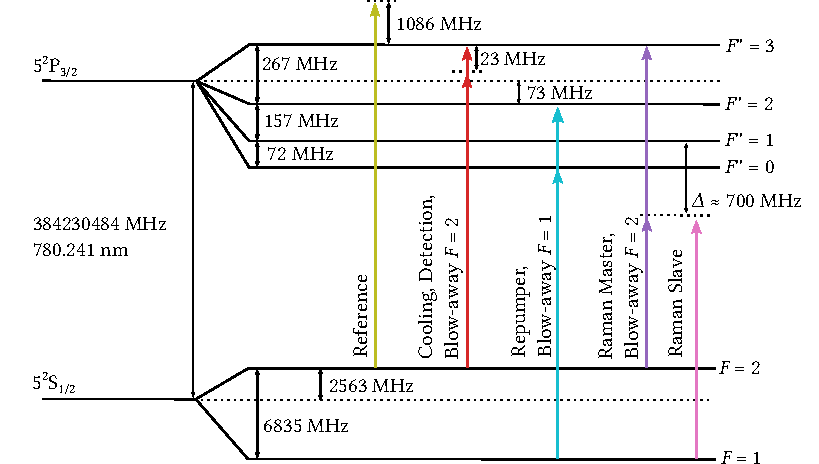
\includegraphics{laser_freqs.pdf}
	\caption{Created with Inkscape}
	\label{fig:laser_freqs}
\end{figure}


This was used to draw fig. \ref{fig:laser_freqs}.




\section{Usage of different mathematics environments}
 {\AmS}-{\LaTeX} is a series of document classes and environments for typesetting mathemtics. The package \code{mathtools} extends this functionality and contains some fixes.

Gl.\,\ref{eq:equation} is a simple equation,
\begin{equation}\label{eq:equation}
	a = b
\end{equation}
Such equations can be split:
\begin{equation}
	\begin{split}
		a& = b+c-d\\
		& \quad + e - f\\
		& = g+h\\
		& = i
	\end{split}
\end{equation}

An expression that spans multiple lines:

\begin{multline}
	a + b + c +d + e + f + a + b + c +d + e + f \\
	+ g + h + i + j + k + l + m + n+ g + h + i + j + k + l + m + n
\end{multline}
And an aligned equation block:
\begin{align}
	a_{11} & = b_{11}          &
	a_{12} & = b_{12}          & \\
	a_{21} & = b_{21}          &
	a_{22} & = b_{22} + c_{22}
\end{align}

\section{More math packages}
Here, we show the usage of some other packages.
\subsection{Differential equations}
With \code{propd} it is possible to typeset differential equations and operators:
\begin{gather}
	\od{y}{x}\\
	\od[2]{u}{x} = -\omega^2 u\\
	\pd{u}{t} = 6u \pd{u}{x} - \pd[3]{u}{x}\\
	\pd{u}{x,x,t}\\
	\pd{}{z}{x+y}\\
	\pd{!}{x}
\end{gather}

\subsection{Chemical formulae}
The package \code{mhchem} is useful to typeset chemical formulae, like \ce{^{235}_{92}U}.

\subsection{Bras and Kets}
For quantum mechanics, use the \code{braket} package:
Quantenmechanik:
\begin{gather}
	\bra{\Phi}\\
	\ket{\Psi}\\
	\braket{\psi|\hat{H}|\phi}
\end{gather}

\subsection{Units}
\code{siunitx} is very useful. It typesets units upright and keeps the appropriate spacing to the value. It is also convenient to specify uncertainties. Here are some examples:

\begin{gather}
	\hbar = \SI[separate-uncertainty=false]{6.62606957(29)e-34}{\joule\second}\\
	g = \SI{9.81(1)}{\meter \per \s^2}\\
	\pi \equiv 3\\
	i \neq \i\\
	e = \SI{1.60217657e-19}{\coulomb}\\
	\e \approx \num{2.71828}\\
\end{gather}
